\subsection{Åbning og Lukning}

Her kommer nu et eksempel på både en åbning og lukning. Figur~\ref{fig:a} er den originale figur.

\begin{figure}[H]
	\centering
	
\includegraphics[width=0.9\linewidth]{figs/spm09/a}
	\caption{Original figur.}
	\label{fig:a}
\end{figure}

\subsubsection{Eksempel på åbning}

Først laves en erosion, som vist på Figur~\ref{fig:a-open-b}.

\begin{figure}[H]
	\centering
	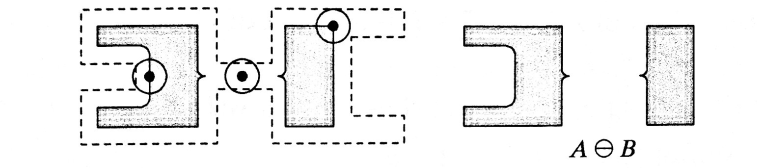
\includegraphics[width=0.9\linewidth]{figs/spm09/a-open-b}
	\caption{Erosion med B på A.}
	\label{fig:a-open-b}
\end{figure}

Så laves en dilation, som vist på Figur~\ref{fig:a-open-b-done}.

\begin{figure}[H]
	\centering
	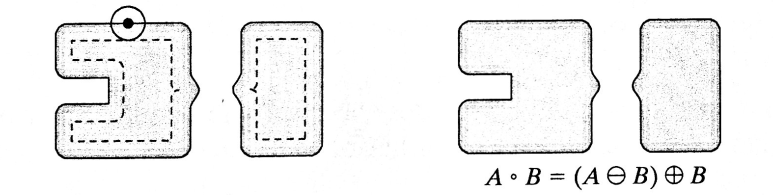
\includegraphics[width=0.9\linewidth]{figs/spm09/a-open-b-done}
	\caption{Færdig åbning. Afsluttet med en dilation.}
	\label{fig:a-open-b-done}
\end{figure}

I dette kan det ses hvordan den tynde forbindelse er fjernet og hvordan de ellers lidt udstikkende ender, som var til højre i det originale billede, også er fjernet.

\subsubsection{Eksempel på lukning}

Først laves en dilation, som vist på Figur~\ref{fig:a-close-b}.

\begin{figure}[H]
	\centering
	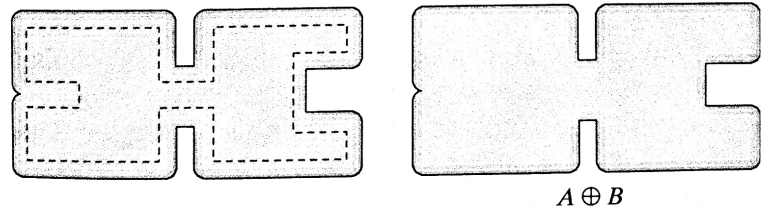
\includegraphics[width=0.9\linewidth]{figs/spm09/a-close-b}
	\caption{Dilation med B på A.}
	\label{fig:a-close-b}
\end{figure}

Så laves en erosion, som vist på Figur~\ref{fig:a-close-b-done}.

\begin{figure}[H]
	\centering
	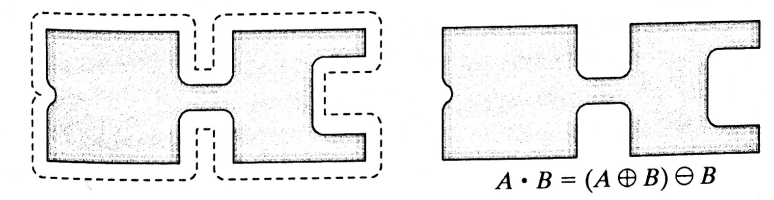
\includegraphics[width=0.9\linewidth]{figs/spm09/a-close-b-done}
	\caption{Færdig lukning. Afsluttet med en erosion.}
	\label{fig:a-close-b-done}
\end{figure}

Her ses det hvordan lukningen på en måde at fuget hjørnerne lidt. Desuden er hullet til venstre i det originale billedet også næsten forsvundet.
